%%%%%%%%%%%%%%%%%%%%%%%%%%%%%%%%%%%%%%%%%%%%%%%%%%%%%%%%%%%%%%%%%%%
%TO AVOID FORMATTING ISSUES, COMPILE THIS ONLY AT WWW.OVERLEAF.COM%
%%%%%%%%%%%%%%%%%%%%%%%%%%%%%%%%%%%%%%%%%%%%%%%%%%%%%%%%%%%%%%%%%%%

%%%%%%%%%%%%%%%%%%%%%%%%%%%%%%%%%%%%%%%%%%%%%%%%%%%%%%%%%%%%%%%%%%%
\documentclass[a4paper,12pt]{article}
\usepackage{graphicx}
%To use this font, you need XeTex or LuaTex, prefer openleaf
\newenvironment{codeblock}{\fontfamily{ccr}\selectfont}{\par}

\title{
	\normalfont \normalsize 
	\textsc{Pimpri Chinchwad College of Engineering \\ 
		Computer Laboratory - IV} \\
	[10pt]   
	\rule{\linewidth}{0.5pt} \\[6pt] 
	\huge Assignment No - A1 \\
	\rule{\linewidth}{2pt}  \\[10pt]
}
\author{}
\date{\normalsize}


\begin{document}
\maketitle

%%%%%%%%%%%%%%%%%%%%%%%
% FOR A NUMBERED LIST
% \begin{enumerate}
% \item Your_Item
% \end{enumerate}
%%%%%%%%%%%%%%%%%%%%%%%
% FOR A BULLETED LIST
% \begin{itemize}
% \item Your_Item
% \end{itemize}
%%%%%%%%%%%%%%%%%%%%%%%
% TO IMPORT AN IMAGE
% \includegraphics[width=\textwidth]{name_of_file}
% \textwidth makes the picture the width of the paragraphs
%%%%%%%%%%%%%%%%%%%%%%%%%%%%%%
% TO CREATE A FIGURE WITH A NUMBER AND CAPTION
% \begin{figure}
% \includegraphics[width=\textwidth]{image}
% \caption{Your Caption Goes Here}
% \label{your_label}
% \end{figure}
% REFER TO YOUR FIGURE LATER WITH
% \ref{your_label}
% LABELS NEED TO BE ONE WORD
%%%%%%%%%%%%%%%%%%%%%%%%%%%%%
% TO ADD CODE
% \begin{codefont}
% Some code in "courier" font
%\end{codefont}
%%%%%%%%%%%%%%%%%%%%%%%%%%%%%
\section{Aim}
	\paragraph{} Using Divide and Conquer Strategies and object-oriented software design technique using Modelio to
	design a software function for Binary Search for an un-ordered data stored in memory. Use necessary
	USE-CASE diagrams and justify its use with the help of mathematical modeling and related efficiency.
	Implement the design using Eclipse C++ or python.
	
\section{Objective}
	\begin{itemize}
		\item To study binary search algorithm
		\item To model the system using Use Case and Class Diagram
	\end{itemize}
	
\section{Software Requirements}
	\begin{itemize}
		\item	Linux Operating System
		\item	GCC
		\item	Umbrello
	\end{itemize}
	
\section{Mathematical Model}
	Let S = {s, e, x, y, Fm,  Si, DD, NDD, memshared}\\
	\\
	s = Initial state, i.e. initialization\\
	e = End state, i.e. minimumm path cost\\
	Si = Intermediate states\\
	Si = {S1, S2,  S3}\\
	S1 = login credentials\\
	S2 = perform operation\\
	S3 = binary search\\
	\\
	X = Input Values\\
	X = {x1, x2}\\
	x1 = Login credentials\\
	x2 = Book details\\
	\\
	Y = Output Values\\
	Y = {y1, y2}\\
	y1 = Requested book\\
	y2 = Failure\\
	\\
	Fm = Main function or algorithm that gives specific output, i.e. main() function.\\
	\\
	NDD = Non deterministic data\\ 
	DD = Deterministic data\\
	Memshared = Core that is used for execution\\
	
\section{Theory}
	\subsection{Divide and Conquer}
		\paragraph{} Divide and conquer (D\&C) is an algorithm design paradigm based on multi-branched recursion. A divide and conquer algorithm works by recursively breaking down a problem into two or more sub-problems of the same (or related) type (divide), until these become simple enough to be solved directly (conquer). The solutions to the sub-problems are then combined to give a solution to the original problem.
		\paragraph{} This divide and conquer technique is the basis of efficient algorithms for all kinds of problems, such as sorting (e.g., quicksort, merge sort), multiplying large numbers (e.g. Karatsuba), syntactic analysis (e.g., top-down parsers), and computing the discrete Fourier transform (FFTs).Advantages of D\&C are : solving difficult problems,Algorithm efficiency,Parallelism,Memory access,etc.
	
	\subsection{Binary Search}
		\paragraph{} The binary search algorithm begins by comparing the target value to the value of the middle element of the sorted array. If the target value is equal to the middle element's value, then the position is returned and the search is finished. If the target value is less than the middle element's value, then the search continues on the lower half of the array; or if the target value is greater than the middle element's value, then the search continues on the upper half of the array. This process continues, eliminating half of the elements, and comparing the target value to the value of the middle element of the remaining elements - until the target value is either found.
		\paragraph{} Divide and conquer strategy used in Binary Search by dividing the set into halves.The conquer part is determining whether and on what position in the processed part there is a searched element.
		
\section{Algorithm}
	\begin{codeblock}
	\# Returns index of x in arr if present, else -1
	def binarySearch (arr, l, r, x):\\
	\\
	\# Check base case\\
	if r $>$= l:\\
	\\
	mid = l + (r - l)/2\\
	\\
	\# If element is present at the middle itself\\
	if arr[mid] == x:\\
	return mid\\
	\\
	\# If element is smaller than mid, then it can only\\
	\# be present in left subarray\\
	elif arr[mid] $>$ x:\\
	return binarySearch(arr, l, mid-1, x)\\
	\\
	\# Else the element can only be present in right subarray\\
	else:\\
	return binarySearch(arr, mid+1, r, x)\\
	\\
	else:\\
	\# Element is not present in the array\\
	return -1\\
	\end{codeblock}



\section{Testing}
\subsection{BLACK BOX TESTING : }
		 Black-box testing is a method of software testing that examines the functionality of an application based on the specifications. It is also known as Specifications based testing. Independent Testing Team usually performs this type of testing during the software testing life cycle.This method of test can be applied to each and every level of software testing such as unit, integration, system and acceptance testing.\\
		 Black box testing techniques are :\\
1) Equivalence Class Partitioning\\
2) Boundary Value Analysis\\
3) Decision Tables\\
4) State Transition Diagrams (or) State Transition Diagrams\\
5) Orthogonal Arrays\\
6) All Pairs Technique\\

\subsection{WHITE BOX TESTING :}
		 White Box Testing (WBT) is also known as Code-Based Testing or Structural Testing. White box testing is the software testing method in which internal structure is being known to tester who is going to test the software. In this method of testing the testcases are calculated based on analysis internal structure of the system based on Code coverage, branches coverage, paths coverage, condition Coverage etc. Typically such method are used at Unit Testing of the code but this different as Unit testing done by the developer \& White Box Testing done by the testers, this is learning the part of the code \& finding out the weakness in the software program under test.
For tester to test the software application under test is like a white/transparent box where the inside of the box is clearly seen to the tester (as tester is aware/access of the internal structure of the code), so this method is called as White Box Testing.

The White-box testing is one of the best method to find out the errors in the software application in early stage of software development life cycle. In this process the deriving the test cases is most important part. The test case design strategy include such that all lines of the source code will be executed at least once or all available functions are executed to complete 100 percent  code coverage of testing. For this, we will use Flow Graphs. Flow graphs are, Syntactic abstraction of source code Resembling to classical flow charts Forms the basis for white box test case generation principles.Conventions of flow graph notation. \\
Why and When White-Box Testing:\\
White box testing is mainly used for detecting logical errors in the program code. It is used for
debugging a code, finding random typographical errors, and uncovering incorrect programming
assumptions .
White box testing is done at low level design and implementable code. It can be applied at all levels of
system development especially Unit, system and integration testing. White box testing can be used for
other development artefacts like requirements analysis, designing and test cases .
White box testing techniques are:\\
1. Static white box testing\\
a. Desk checking\\
b. Code walkthrough\\
c. Formal Inspections\\
2. Structural White box testing\\
a. Control flow/ Coverage testing\\
b. Basic path testing\\
c. Loop testing\\
d. Data flow \\


Sample Input: For integer array int A[] = 1,2,3,4,5,6,7,8,9,10; Function 
is passed\\
following arguments: Binary Search(A, 1, 10, 7);\\
Output obtained: Entered second Entered third Entered first 6\\
The underlined nodes are the ones being tested. The above output shows
that every test region is covered for given input.\\

	\begin{figure}[h!]
		\centering
		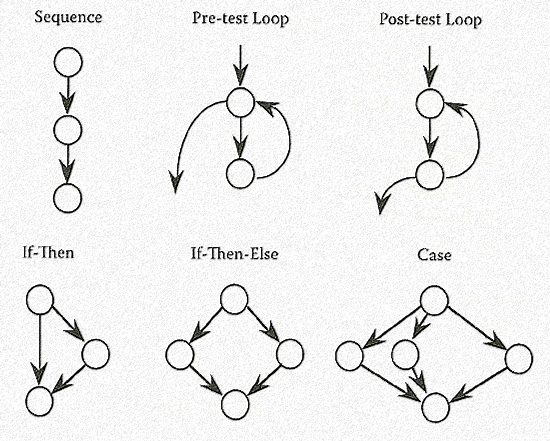
\includegraphics[scale=0.30]{CFG.png}
	\end{figure}

\subsection{ POSITIVE/NEGATIVE TESTING }

\textbf{Positive Testing :}\\
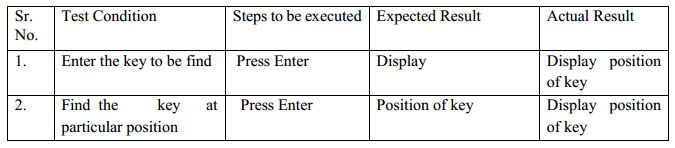
\includegraphics[width=\textwidth]{binary_positive}
\vspace{30px}

\textbf{Negative Testing :}\\
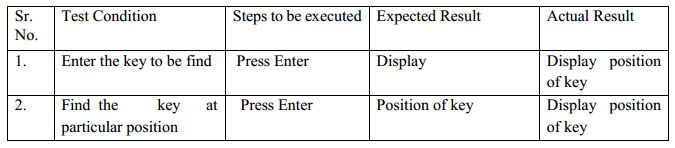
\includegraphics[width=\textwidth]{binary_positive}

\newpage

\section{Use Case Diagram}
	\begin{figure}[h!]
		\centering
		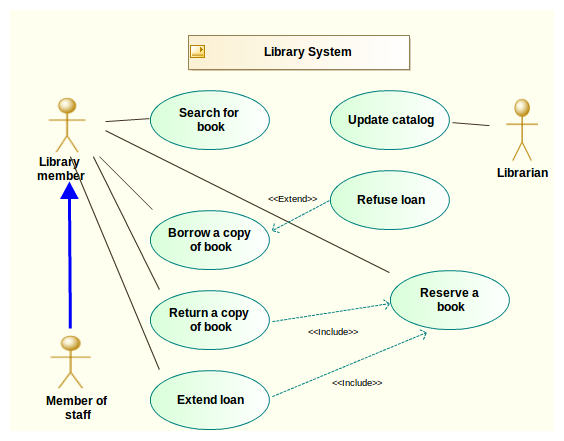
\includegraphics[scale=0.50]{use_case.png}
		\caption{Use Case Diagram}
		\label{Use Case Diagram}
	\end{figure}

\section{Class Diagram}
	
\begin{figure}[htb!]
		\centering
		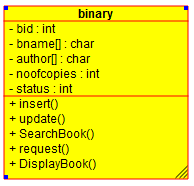
\includegraphics[scale = 0.80]{bst-class}
		\caption{Class Diagram}
		\label{Class Diagram}
		\end{figure}

\newpage

\section{Activity Diagram}
	
\begin{figure}[htb!]
		
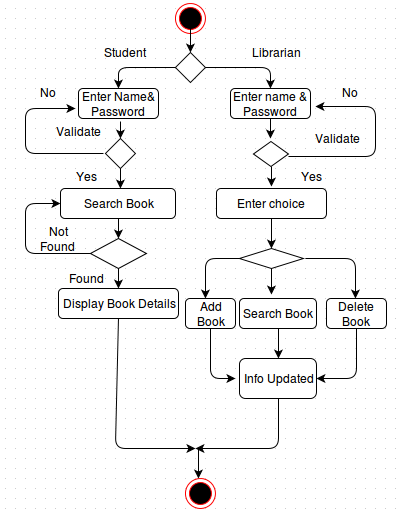
\includegraphics[scale = 0.80]{aaaa}
		\centering
		\caption{Activity Diagram}
		\label{Activity Diagram}
		\end{figure}



\section{Conclusion}
	\paragraph{} Thus we have successfully used Divide and Conquer Strategies and object-oriented software design technique using Modelio to design a software function for Binary Search for an un-ordered data stored in memory.
\vspace{20px}


\begin{center}
	\begin{tabular}
		{|c|c|c|c|}\hline
		{\bf Roll No.}		&{\bf  Name of Student}		  				&{\bf Date of Submission}  \\ \hline
		{302}	&	{Abhinav Bakshi}	& {21/12/15}  \\ \hline
	\end{tabular}\\ 
\end{center}
\newpage


\begin{figure}[htb!]
	\centering
	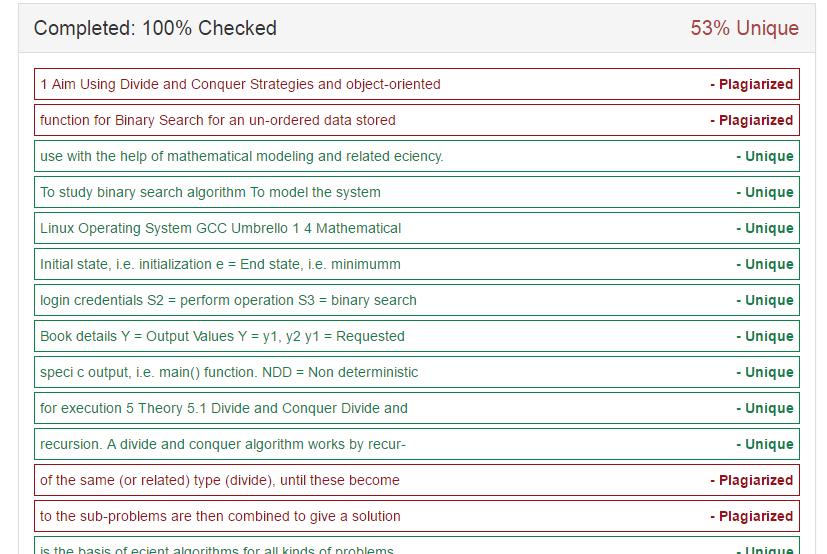
\includegraphics[scale = 0.80]{Untitled.png}
	\caption{Plagiarism Report }
	\label{Plagiarism Report}
\end{figure}



\end{document}
 

 

